%%%%%%%%%%%%%%%%%%%%%%%%%%%%%%%%
\section{Battery Systems for Electric Vehicles} \label{sec:battery}
%%%%%%%%%%%%%%%%%%%%%%%%%%%%%%%%

%\abstract
Battery systems are an important part of electric vehicles.  The main research areas in battery system are modeling, simulation, estimation and optimization. In the following, literature survey of battery systems for electric vehicles is presented. 

%%%%%%%%%%%%%%%%%%%%%%%%%%%%%%%%
\subsection{Modeling}

Rechargeable batteries that offer high energy and
power density and relative safety are the choice for many applications from consumer
electronics to electric vehicles. One example of such batteries are Lithium-ion batteries. Modeling the cycle and
calendar life of such batteries is needed to set
expectations of reliable product performance. Generally, there are two types of models to predict the battery life~\cite{ZS_millner}. One type of models describe chemistry of the cell~\cite{ZS_Ning}. These models, with the help of extensive computation facilities, provide time and temperature effects accurately but do not match with cycle life test data. Such models are best suited for
optimization of the physical design aspects of electrodes
and electrolyte~\cite{ZS_den}. The other type is empirical models~\cite{ZS_dubarry} that fit the test data to equivalent circuit models using power law relationships. These models have limited range of parameters and require extensive testing of each type of cells. 

A simple battery model consists of an ideal battery with an open circuit voltage and and a constant internal series resistance. A new battery model based on simple battery model was proposed in~\cite{ZS_jean}. In this battery model, SoC (State of Charge) of the battery is considered as well by making the internal resistance variable. Another commonly used model is the Thevenin battery
model in Fig.~\ref{fig:ZS_battery_model}, which consists of an ideal no-load battery voltage ($E_o$),
internal resistance ($R$), capacitance ($C_o$) and overvoltage
resistance ($R_o$)~\cite{ZS_salameh}. $C_o$ represents the capacitance of the parallel
plates and $R_o$ represents the non-linear resistance contributed
by the contact resistance of plate to electrolyte. The main disadvantage of the Thevenin battery model is that
all the elements are assumed to be constant, but in fact all the
values are functions of battery conditions.


\begin{figure}[b]
\centering
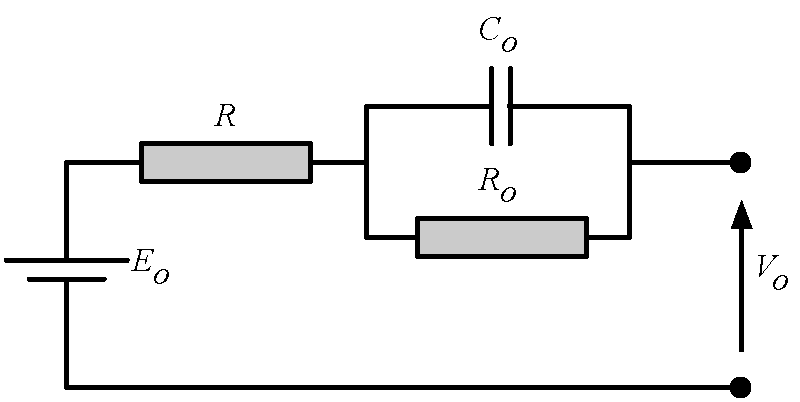
\includegraphics[scale=0.5]{Figures/Zili_Shao/ZS_figure1.pdf}
\caption{Thevenin battery model~\cite{ZS_salameh}.}
\label{fig:ZS_battery_model}
\end{figure}

An empirical mathematical model is developed in \cite{ZS_jayne,ZS_sims}. The improvement of this model is to account for the nonlinear
characteristic of both the open circuit voltage and
internal resistance. A sophisticated and accurate dynamic model for simulation purpose was proposed in \cite{ZS_gig}. This model includes electrolyte reaction, Ohmic effect and leakage capacitance as well as the self discharge current. The drawbacks of this model include longer time for computation because of its higher order and complicated modeling procedure that involves a lot of empirical data. Another battery model is called over-current battery model as described in \cite{ZS_rob}. It has a variable
current source, a variable voltage source, a variable resistor, and a capacitor. 
This model provides a good representation of both variable
internal drop in the battery and changes in the output voltage
due to the SoC. However, one of its drawbacks is
that too many parameters are required. A model described in \cite{ZS_zi,ZS_mar}
considers most nonlinear battery element characteristics both during charging and 
discharging as well as their dependence on the SoC of the battery. All the elements included in this model are functions of the
open-circuit voltage of a battery, which in turn relates to state of
charge~\cite{ZS_chan}.


The model in \cite{ZS_chen} is capable of predicting run time and I-V performance, but is not
accurate for the transient response to short-duration loads. As a result, it does not predict accurately
the SoC throughout drive cycles for electric-vehicle-related simulations \cite{ZS_kro}. A model proposed in \cite{ZS_kro} describes accurate determination of the discharge capacity, which is a function of the discharge rate, temperature, cycle number, and a rate factor that accounts
for a decrease in capacity due to unwanted side reactions
 as the current increases. This model can also predicts SoC, terminal voltage and power losses of various batteries for electric vehicles. Along with predicting the battery behavior accurately, this model can be used for simulation as well. 
 
%%%%%%%%%%%%%%%%%%%%%%%%%%%%%%%%
\subsection{Simulation}

Simulation with an accurate battery model is able to analyze complex phenomena. Average ratings can be
derived from steady-state operation and characteristics of the
system, but peak ratings can only be estimated from the steady state results and are often inadequate. A detailed model is appropriate for short-term
analysis and supplements the long-term capabilities of a
steady-state model as described in \cite{ZS_wip,ZS_adv}.  In order to better understand losses, thermal
characteristics, and durability of various  electric vehicle batteries, a
dynamic simulator is a key tool. Estimates of conducting losses in
power electronics devices, batteries, supercapacitors, and other components can be supported directly with a dynamic model. 
%The ADVISOR program developed through the National Renewable Energy Laboratory (NREL) \cite{ZS_bai} is a simulator based on static maps that reflects steady-state behavior of vehicle subsystems. 
Dynamic models are needed to make lower-level comparisons
among subsystems and support subsystem design. Steady-state simulation tools for the design and analysis of
hybrid electric automotives have been developed in recent years and support comparisons over long drive cycles. In the past, dynamic
simulation models have focused mainly on the analysis of
control strategies \cite{ZS_amr}. A dynamic simulator in \cite{ZS_log} offers a more
detailed look, based on dynamic equations of each
subcomponent (the engine, battery, inverter, motor, and
transmission) on microsecond time scales.

Several simulation systems have been
developed to describe the operation of hybrid electric power
trains such simple electric vehicle simulation (SIMPLEV) from
the DOE’s Idaho National Laboratory \cite{ZS_col}. Simulation programs include MARVEL from
Argonne National Laboratory \cite{ZS_wal}, CarSim from AeroVironment
Inc., JANUS from Durham University \cite{ZS_bum}, 
%ADVISOR from the DOE’s National Renewable Energy Laboratory \cite{ZS_wip},
Vehicle Mission Simulator \cite{ZS_noo}, and others \cite{ZS_aue,ZS_kri}. A
simulation model (ELPH) is used to study the viability of an electrically
peaking control scheme and to determine the applicability of
computer modeling to electric vehicle design \cite{ZS_bun}. V-Elph \cite{ZS_ste,ZS_but} is a system-level modeling, simulation,
and analysis package. This package uses Matlab/Simulink to study issues related to electric vehicle and
hybrid electric vehicle design such as energy efficiency, fuel economy, and
vehicle emissions. V-Elph facilitates in-depth study of power
plant configurations, component sizing, energy management
strategies, and the optimization of important component parameters
for several types of hybrid or electric configuration
or energy management strategies with visual programming
techniques, allowing the user to quickly change architectures,
parameters, and to view output data graphically~\cite{Butler:TVT99}.

%%%%%%%%%%%%%%%%%%%%%%%%%%%%%%%%
\subsection{Estimation}

Automotive Lithium-ion batteries have high capacity and large serial parallel
numbers, which, coupled with the problems such as safety,
durability, uniformity and cost, imposes limitations on the wide
application of lithium-ion batteries in vehicles. Lithium-ion
batteries must operate within the safe and reliable operating area, which is restricted by temperature and voltage windows. Exceeding the restrictions of these windows will lead to rapid
attenuation of battery performance and even result in safety
problems \cite{ZS_lu}. The accommodation
of such operating conditions requires that a management system has accurate knowledge of  many factors e.g. the  SoC to facilitate safe and efficient operation.
Failure to control SoC, which may lead to under- or over-charging
conditions, can degrade the ability of the pack to source/sink
subsequent power transients \cite{ZS_bha}.

A variety of techniques have been proposed to measure or
monitor the SoC of a cell or battery, each having its relative
merits \cite{ZS_pil}. Coulomb counting or current
integration is, at present, the most commonly used technique,
requiring dynamic measurement of the cell/battery current,
the time integral of which is considered to provide a direct
indication of SoC \cite{ZS_cau}. 

 Due to complexity of electrochemical processes in batteries and noise in sensors, many sophisticated algorithms have been proposed for efficient battery monitoring, such as estimation of SoC \cite{ZS_cun}. An  earlier  work  which  uses  voltage  as  the  basis  of  SoC estimation is presented in \cite{ZS_ver}. Though this work deals with complexities  such  as  hysteresis,  it  is difficult to estimate SoC for some battery types such as Nickel-metal  hybrid.  A  fuzzy  logic  approach  for  SoC  estimation is  presented  in \cite{ZS_sin}. This approach  requires  training  data, which is  challenging  because  of  changing  properties  in  different conditions.  A  complex  neural-network-based  approach  is presented in \cite{ZS_ang}, but it is restricted to lead acid batteries and requires complex network design and computation. 
 
 A hybrid neural-network and genetic-algorithm based approach of SoC estimation  of  series  connected  modules  (battery  cells)  is discussed in \cite{ZS_11}. Despite the promising result, the proposed method is relatively complex and has high computational cost. In \cite{ZS_12}, a complicated mathematical model has been devised, specifically for lead acid batteries, which can predict the SoC and remaining operation time with up to 10\% error. A nonlinear estimation method based on the sliding mode observer is presented in \cite{ZS_13}. This work also discusses the parameters of the  battery  model  through  different  tests.  A  novel  algorithm is  presented  in \cite{ZS_14}, which  combines  the  weighted  sum  of complex  voltage  based  methods  and Coulomb  counting  techniques.  An  earlier  method  based  on Kalman  filter  is  presented  in \cite{ZS_15,ZS_16,ZS_17,ZS_18}.  In  addition  to  a few similar methods, a famous estimation algorithm based on Extended Kalman Filter is proposed in \cite{ZS_19,ZS_20,ZS_21,ZS_22,ZS_23,ZS_24} and has shown promising results. The method proposed in \cite{ZS_shaheer} can robustly estimate SoC by using simple but accurate battery models employing a conservative filtering technique. The $H_\infty$ filter is  solved  optimally  by  formulating  it  as  a Linear Matrix Inequality problem. The separation of computation (calculation of gain once and iterative implementation of estimator) enables the proposed method to be implemented on embedded controllers without compromising real-time operation requirements.

SoH (state of Health) is a quantifying estimation that reflects the general
condition of a battery and its ability to deliver the specified
performance compared with a fresh battery. Battery
capacity (i.e., the energy storage capacity) has long been the
target of researchers as the definitive battery SoH indicator \cite{ZS_yu}. In general, a lithium battery is deemed to fail when its capacity
fades by 20 \% of the rated value \cite{ZS_pas}.

%%%%%%%%%%%%%%%%%%%%%%%%%%%%%%%%
\subsection{Optimization}

One of the problems for electric vehicle designers is that energy and power density need to be carefully balanced. Heavy batteries increase the vehicle’s range and light batteries increase the power-to-weight ratio, enabling the electric vehicle to achieve better acceleration.
More batteries, however, increase the cost of the vehicle design. 

Electric vehicles do have quick acceleration, due to the high torque of the electric motor. Currently nickel metal hydride (NiMH) and Lithium-ion are the common, though research continues into new battery chemistries, such as nano-phosphate cathodes, to allow for high discharge rates and higher performance. The discharge rate for batteries contributes to not only acceleration rates, but also how quickly the batteries will be charged. The higher the rate, the more energy is lost through heat. Supercapacitors are available as alternative components. They have high charge and discharge rates, resulting in lower losses but these benefits can be outweighed by their low energy density \cite{ZS_coi}.

The charging management concepts can also be divided into
centralized and decentralized approaches \cite{ZS_war}. The decentralized
approaches let the electric vehicles optimize its charging behavior
based on, for example, a price signal broadcast. The drawback
of this approach is that the electric vehicle needs to collect and store the
trip history. If the electric vehicles should coordinate their charging, for
example to include distribution grid constraints, the need for
V2V (Vehicle to vehicle) communication is high. 

The centralized approaches
focus on a centralized unit that directly controls the charging of electric vehicles. Additional study on forecasting and managing electric vehicle
charging can be found in \cite{ZS_rah,ZS_gal}. A novel method for optimization is presented by \cite{ZS_sun} which describes the method for planing the charging of electric vehicles with electric grid constraints including voltage and power. This method provides an individual charging plan for each vehicle, which helps in avoiding the congestion on distribution grids. Using quadratic approximation approaches to optimize the behavior electrical vehicle battery, the goals of minimizing charging costs, achieving satisfactory state of energy levels and optimal power balancing have been achieved \cite{ZS_sun2}.

